\documentclass{standalone}
\usepackage{tikz}
\usetikzlibrary{patterns, positioning}
\usepackage[sfdefault]{ClearSans} %% option 'sfdefault' activates Clear Sans as the default text font
\usepackage[T1]{fontenc}

\begin{document}
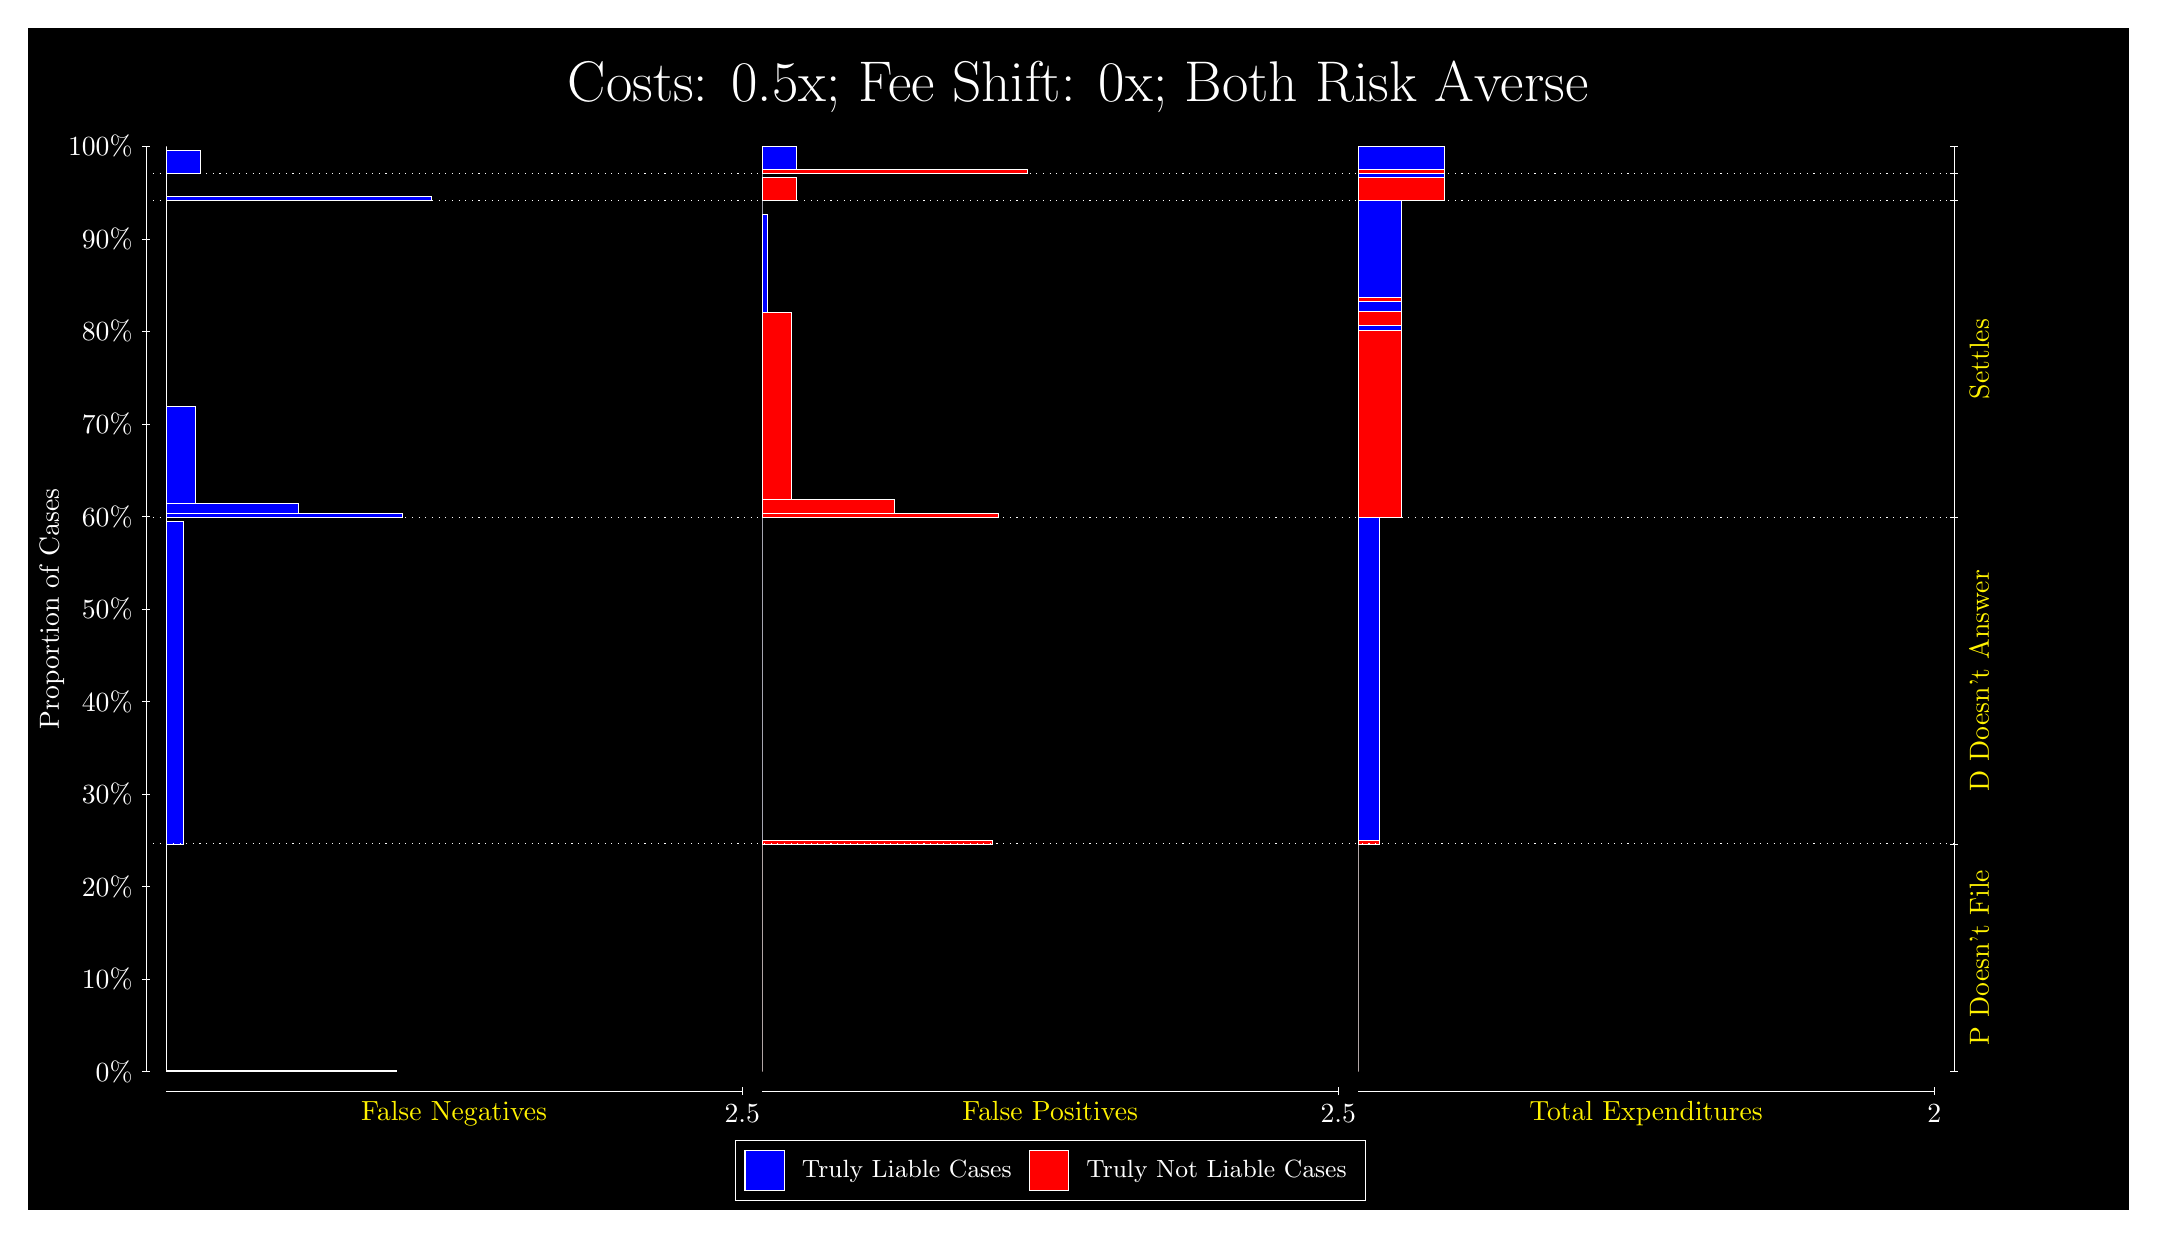
\begin{tikzpicture}
\draw[fill=black] (0,0) rectangle (26.667,15);
\draw[text=white] (0,13.5) rectangle (26.667,15) node[midway] {\huge Costs: 0.5x; Fee Shift: 0x; Both Risk Averse};
\draw[white, very thin] (1.5,1.75) -- (1.5,13.5);
\node[rotate=90, text=white, anchor=center] at (0.3, 7.625) {Proportion of Cases};
\draw[white, very thin] (1.45,1.75) -- (1.55,1.75);
\node[text=white, anchor=east] at (1.45, 1.75) {0\%};
\draw[white, very thin] (1.45,2.925) -- (1.55,2.925);
\node[text=white, anchor=east] at (1.45, 2.925) {10\%};
\draw[white, very thin] (1.45,4.1) -- (1.55,4.1);
\node[text=white, anchor=east] at (1.45, 4.1) {20\%};
\draw[white, very thin] (1.45,5.275) -- (1.55,5.275);
\node[text=white, anchor=east] at (1.45, 5.275) {30\%};
\draw[white, very thin] (1.45,6.45) -- (1.55,6.45);
\node[text=white, anchor=east] at (1.45, 6.45) {40\%};
\draw[white, very thin] (1.45,7.625) -- (1.55,7.625);
\node[text=white, anchor=east] at (1.45, 7.625) {50\%};
\draw[white, very thin] (1.45,8.8) -- (1.55,8.8);
\node[text=white, anchor=east] at (1.45, 8.8) {60\%};
\draw[white, very thin] (1.45,9.975) -- (1.55,9.975);
\node[text=white, anchor=east] at (1.45, 9.975) {70\%};
\draw[white, very thin] (1.45,11.15) -- (1.55,11.15);
\node[text=white, anchor=east] at (1.45, 11.15) {80\%};
\draw[white, very thin] (1.45,12.325) -- (1.55,12.325);
\node[text=white, anchor=east] at (1.45, 12.325) {90\%};
\draw[white, very thin] (1.45,13.5) -- (1.55,13.5);
\node[text=white, anchor=east] at (1.45, 13.5) {100\%};

\draw[white, very thin] (24.457,1.75) -- (24.457,13.5);
\draw[white, very thin] (24.407,1.75) -- (24.507,1.75);
\node[anchor=west] at (24.407, 1.75) {};
\draw[white, very thin] (24.407,4.6417) -- (24.507,4.6417);
\node[anchor=west] at (24.407, 4.6417) {};
\draw[white, very thin] (24.407,8.7832) -- (24.507,8.7832);
\node[anchor=west] at (24.407, 8.7832) {};
\draw[white, very thin] (24.407,12.815) -- (24.507,12.815);
\node[anchor=west] at (24.407, 12.815) {};
\draw[white, very thin] (24.407,13.157) -- (24.507,13.157);
\node[anchor=west] at (24.407, 13.157) {};
\draw[white, very thin] (24.407,13.5) -- (24.507,13.5);
\node[anchor=west] at (24.407, 13.5) {};

\draw[white, very thin, fill=blue] (1.75,1.75) rectangle (4.6775,1.7662);
\draw[white, very thin, fill=red] (1.75,1.7662) rectangle (1.75,4.6417);
\draw[white, very thin, fill=blue] (1.75,4.6417) rectangle (1.9696,8.7413);
\draw[white, very thin, fill=red] (1.75,8.7413) rectangle (1.75,8.7832);
\draw[white, very thin, fill=blue] (1.75,8.7832) rectangle (4.7507,8.846);
\draw[white, very thin, fill=blue] (1.75,8.846) rectangle (3.4333,8.9649);
\draw[white, very thin, fill=blue] (1.75,8.9649) rectangle (2.1159,10.2);
\draw[white, very thin, fill=red] (1.75,10.2) rectangle (1.75,12.815);
\draw[white, very thin, fill=blue] (1.75,12.815) rectangle (5.1167,12.862);
\draw[white, very thin, fill=red] (1.75,12.862) rectangle (1.75,13.157);
\draw[white, very thin, fill=blue] (1.75,13.157) rectangle (2.1891,13.452);
\draw[white, very thin, fill=red] (1.75,13.452) rectangle (1.75,13.5);
\draw[white, very thin, fill=red] (9.3189,1.75) rectangle (9.3189,4.6254);
\draw[white, very thin, fill=blue] (9.3189,4.6254) rectangle (9.3189,4.6417);
\draw[white, very thin, fill=red] (9.3189,4.6417) rectangle (12.246,4.6836);
\draw[white, very thin, fill=blue] (9.3189,4.6836) rectangle (9.3189,8.7832);
\draw[white, very thin, fill=red] (9.3189,8.7832) rectangle (12.32,8.8369);
\draw[white, very thin, fill=red] (9.3189,8.8369) rectangle (11.002,9.0134);
\draw[white, very thin, fill=red] (9.3189,9.0134) rectangle (9.6848,11.398);
\draw[white, very thin, fill=blue] (9.3189,11.398) rectangle (9.3921,12.633);
\draw[white, very thin, fill=blue] (9.3189,12.633) rectangle (9.3189,12.815);
\draw[white, very thin, fill=red] (9.3189,12.815) rectangle (9.758,13.11);
\draw[white, very thin, fill=blue] (9.3189,13.11) rectangle (9.3189,13.157);
\draw[white, very thin, fill=red] (9.3189,13.157) rectangle (12.686,13.205);
\draw[white, very thin, fill=blue] (9.3189,13.205) rectangle (9.758,13.5);
\draw[white, very thin, fill=red] (16.888,1.75) rectangle (16.888,4.6254);
\draw[white, very thin, fill=blue] (16.888,4.6254) rectangle (16.888,4.6417);
\draw[white, very thin, fill=red] (16.888,4.6417) rectangle (17.162,4.6836);
\draw[white, very thin, fill=blue] (16.888,4.6836) rectangle (17.162,8.7832);
\draw[white, very thin, fill=red] (16.888,8.7832) rectangle (17.437,11.168);
\draw[white, very thin, fill=blue] (16.888,11.168) rectangle (17.437,11.231);
\draw[white, very thin, fill=red] (16.888,11.231) rectangle (17.437,11.407);
\draw[white, very thin, fill=blue] (16.888,11.407) rectangle (17.437,11.526);
\draw[white, very thin, fill=red] (16.888,11.526) rectangle (17.437,11.58);
\draw[white, very thin, fill=blue] (16.888,11.58) rectangle (17.437,12.815);
\draw[white, very thin, fill=red] (16.888,12.815) rectangle (17.986,13.11);
\draw[white, very thin, fill=blue] (16.888,13.11) rectangle (17.986,13.157);
\draw[white, very thin, fill=red] (16.888,13.157) rectangle (17.986,13.205);
\draw[white, very thin, fill=blue] (16.888,13.205) rectangle (17.986,13.5);
\draw[white, dotted] (1.5,4.6417) -- (24.457,4.6417);
\draw[white, dotted] (1.5,8.7832) -- (24.457,8.7832);
\draw[white, dotted] (1.5,12.815) -- (24.457,12.815);
\draw[white, dotted] (1.5,13.157) -- (24.457,13.157);
\draw[white, very thin] (1.75,1.5) -- (9.0689,1.5);
\node[text=yellow, anchor=north] at (5.4094, 1.5) {False Negatives};
\draw[white, very thin] (9.0689,1.45) -- (9.0689,1.55);
\node[text=white, anchor=north] at (9.0689, 1.45) {2.5};

\draw[white, very thin] (9.3189,1.5) -- (16.638,1.5);
\node[text=yellow, anchor=north] at (12.978, 1.5) {False Positives};
\draw[white, very thin] (16.638,1.45) -- (16.638,1.55);
\node[text=white, anchor=north] at (16.638, 1.45) {2.5};

\draw[white, very thin] (16.888,1.5) -- (24.207,1.5);
\node[text=yellow, anchor=north] at (20.547, 1.5) {Total Expenditures};
\draw[white, very thin] (24.207,1.45) -- (24.207,1.55);
\node[text=white, anchor=north] at (24.207, 1.45) {2};

\node[text=yellow, centered, rotate=90] at (24.777, 3.1958) {P Doesn't File};
\node[text=yellow, centered, rotate=90] at (24.777, 6.7124) {D Doesn't Answer};
\node[text=yellow, centered, rotate=90] at (24.777, 10.799) {Settles};



\draw (12.978300999999998,1.5) node[draw=none] (baseCoordinate) {};
\begin{scope}[align=center]
        \matrix[scale=0.5, draw=white, below=0.5cm of baseCoordinate, nodes={draw}, column sep=0.1cm]{
            \node[rectangle, draw, minimum width=0.5cm, minimum height=0.5cm, fill=blue] {}; &
            \node[draw=none, font=\small, text=white] (B) {Truly Liable Cases}; &
            \node[rectangle, draw, minimum width=0.5cm, minimum height=0.5cm, fill=red] {}; &
            \node[draw=none, font=\small, text=white] (B) {Truly Not Liable Cases}; \\
            };
\end{scope}

\end{tikzpicture}
\end{document}